%
% This is a borrowed LaTeX template file for lecture notes for CS267,
% Applications of Parallel Computing, UCBerkeley EECS Department.
% Now being used for CMU's 10725 Fall 2012 Optimization course
% taught by Geoff Gordon and Ryan Tibshirani.  When preparing 
% LaTeX notes for this class, please use this template.
%
% To familiarize yourself with this template, the body contains
% some examples of its use.  Look them over.  Then you can
% run LaTeX on this file.  After you have LaTeXed this file then
% you can look over the result either by printing it out with
% dvips or using xdvi. "pdflatex template.tex" should also work.
%

\documentclass[twoside]{article}
\setlength{\oddsidemargin}{0.25 in}
\setlength{\evensidemargin}{-0.25 in}
\setlength{\topmargin}{-0.6 in}
\setlength{\textwidth}{6.5 in}
\setlength{\textheight}{8.5 in}
\setlength{\headsep}{0.75 in}
\setlength{\parindent}{0 in}
\setlength{\parskip}{0.1 in}

%
% ADD PACKAGES here:
%

\usepackage{amsmath,amsfonts,graphicx}
\usepackage{graphicx}
\graphicspath{ {./} }

%
% The following commands set up the lecnum (lecture number)
% counter and make various numbering schemes work relative
% to the lecture number.
%
\newcounter{lecnum}
\renewcommand{\thepage}{\thelecnum-\arabic{page}}
\renewcommand{\thesection}{\thelecnum.\arabic{section}}
\renewcommand{\theequation}{\thelecnum.\arabic{equation}}
\renewcommand{\thefigure}{\thelecnum.\arabic{figure}}
\renewcommand{\thetable}{\thelecnum.\arabic{table}}

%
% The following macro is used to generate the header.
%
\newcommand{\lecture}[4]{
   \pagestyle{myheadings}
   \thispagestyle{plain}
   \newpage
   \setcounter{lecnum}{#1}
   \setcounter{page}{1}
   \noindent
   \begin{center}
   \framebox{
      \vbox{\vspace{2mm}
    \hbox to 6.28in { {\bf UCSB CS 291D: Blockchains and Cryptocurrencies
	\hfill Fall 2020} }
       \vspace{4mm}
       \hbox to 6.28in { {\Large \hfill Lecture #1: #2  \hfill} }
       \vspace{2mm}
       \hbox to 6.28in { {\it Lecturer: #3 \hfill Scribes: #4} }
      \vspace{2mm}}
   }
   \end{center}
   \markboth{Lecture #1: #2}{Lecture #1: #2}

%   {\bf Note}: {\it LaTeX template courtesy of UC Berkeley EECS dept.}

%   {\bf Disclaimer}: {\it These notes have not been subjected to the
%   usual scrutiny reserved for formal publications.  They may be distributed
%   outside this class only with the permission of the Instructor.}
%   \vspace*{4mm}
}
%
% Convention for citations is authors' initials followed by the year.
% For example, to cite a paper by Leighton and Maggs you would type
% \cite{LM89}, and to cite a paper by Strassen you would type \cite{S69}.
% (To avoid bibliography problems, for now we redefine the \cite command.)
% Also commands that create a suitable format for the reference list.
\renewcommand{\cite}[1]{[#1]}
\def\beginrefs{\begin{list}%
        {[\arabic{equation}]}{\usecounter{equation}
         \setlength{\leftmargin}{2.0truecm}\setlength{\labelsep}{0.4truecm}%
         \setlength{\labelwidth}{1.6truecm}}}
\def\endrefs{\end{list}}
\def\bibentry#1{\item[\hbox{[#1]}]}

%Use this command for a figure; it puts a figure in wherever you want it.
%usage: \fig{NUMBER}{SPACE-IN-INCHES}{CAPTION}
\newcommand{\fig}[3]{
			\vspace{#2}
			\begin{center}
			Figure \thelecnum.#1:~#3
			\end{center}
	}
% Use these for theorems, lemmas, proofs, etc.
\newtheorem{theorem}{Theorem}[lecnum]
\newtheorem{lemma}[theorem]{Lemma}
\newtheorem{proposition}[theorem]{Proposition}
\newtheorem{claim}[theorem]{Claim}
\newtheorem{corollary}[theorem]{Corollary}
\newtheorem{definition}[theorem]{Definition}
\newenvironment{proof}{{\bf Proof:}}{\hfill\rule{2mm}{2mm}}

% **** IF YOU WANT TO DEFINE ADDITIONAL MACROS FOR YOURSELF, PUT THEM HERE:

\newcommand\E{\mathbb{E}}

\begin{document}
%FILL IN THE RIGHT INFO.
%\lecture{**LECTURE-TITLE**}{**DATE**}{**LECTURER**}{**SCRIBE**}
\lecture{7}{EVM and Solidity Programming}{Shumo Chu}{Harlan Kringen, Jiyu Zhang}
%\footnotetext{These notes are partially based on those of Nigel Mansell.}

% **** YOUR NOTES GO HERE:

% Some general latex examples and examples making use of the
% macros follow.  
%**** IN GENERAL, BE BRIEF. LONG SCRIBE NOTES, NO MATTER HOW WELL WRITTEN,
%**** ARE NEVER READ BY ANYBODY.
This lecture's notes walk through a high-level overview of the Ethereum Virtual
Machine (EVM) and its associated programming language, Solidity.

\section{Architecture and Design of the EVM}

The design of the Ethereum blockchain resembles Bitcoin overall but departs in
its handling of the users' account state.  Whereas Bitcoin employs a UTXO
approach, Ethereum uses a more traditional input/output ledger approach which is
implemented by the blockchain.  In this blockchain model a block has hash
pointers to a world state, transactions, logs, as well as other transaction
blocks.  This may be roughly visualized in the following diagram.

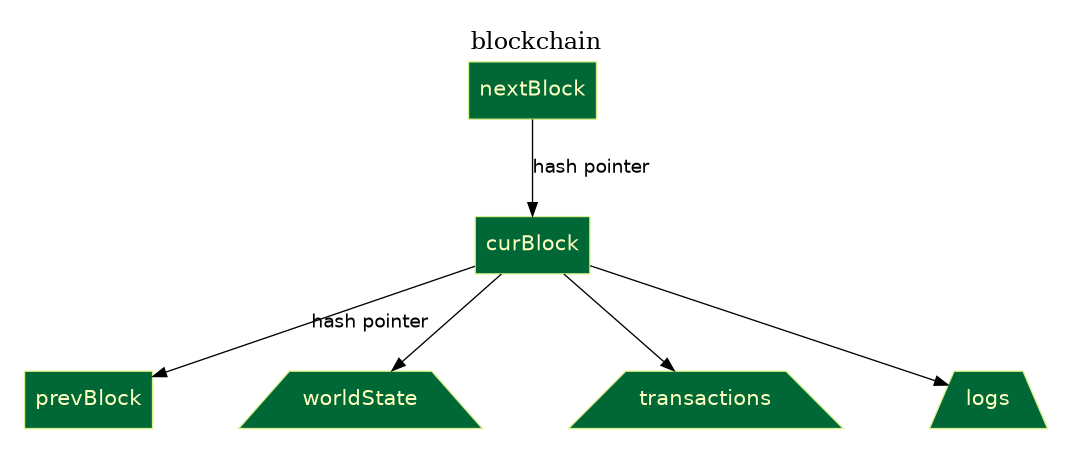
\includegraphics[scale=0.38]{evm}

\subsection{Workflow}

The Ethereum blockchain, like Bitcoin, has the ability to store information
immutably, but it can also run general computations on its blockchain, in the
form of smart contracts, which are simply small programs that can work with any
information committed to the blockchain.

The Ethereum blockchain runs these programs on the Ethereum Virtual Machine
(EVM), which is a stack machine similar to the engine that runs Bitcoin script.
Smart contracts can be written in any language that compiles to EVM bytecode,
however Solidity is the most common.

Every contract, like every transaction, is sent to all miners on Ethereum to be
verified.  The manner in which a contract is successfully verified is somewhat
involved.  First, the miners are rewarded with 2 Ether plus a transaction cost
for every block.  Second, there is an extra layer of payment that is mediated
through the notion of ``gas'' that is unique to Ethereum.  This will be
explained below.  

The EVM itself is not a powerful computer, having about as much computing power
as a smartphone.  Additionally, the EVM stack machine's stack depth is
relatively shallow, capped at 1024 levels.  This contributes to its spartan
computational profile.

\section{Gas and Incentives}

As mentioned in the introduction, the process of verifying a block for the
blockchain requires the willful participation of other miners.  The miners must
spend computational resources to verify a given block, and so the reward for
doing this must be clear and competitive with whatever else the miners could be
using their computational power for. 

Ethereum creates another layer to the incentive system, namely gas.  The concept
of gas, which is decoupled into two subcomponents, gas price and gas limit, is
an amount of Ether (typically denoted in Wei) that approximates the amount of
computational power needed to run a contract.  For a given contract, the EVM
must spend some number of cycles executing and Ethereum attributes to each cycle a
gas price.

As a decoupled notion, gas price is a user-defined primitive that reflects the
user's expectation of how much computational power will be required to run the
contract.  The gas limit is a ceiling on how much the gas price may be, which is
simply another check on users abusing the stack machine's (and miners')
computational power.  The total cost of a transaction is $gasPrice * gasLimit$,
and the fee paid to the miner is the total amount of gas needed to run the
contract multiplied by the gasPrice and any leftover gas is returned to the
user.

If the gas price for a contract is larger than the amount of gas needed to run
the contract, the difference will be refunded to the user.  The gas itself then
pays the miners who worked to verify the block.  If the gas price is
insufficient, this will trigger a runtime error and the contract itself will not
be added to the blockchain, although gas spent on the contract will still go to
the miners involved.

There are of course problems inherent in the concept of gas.  Because it is
dynamically computed, a user can only make an educated guess at how much gas a
contract will require.  Even worse, if a contract invokes other contracts, the
problem of estimating gas usage is compounded in a non-obvious way.  We can see
this in the below diagram.

Ultimately gas serves a dual purpose.  In the first case gas adds another
mechanism for miners and users to leverage in order to commit their blocks to
the blockchain, by, for instance, setting a competitive and attractive gas
price.  In the second case, gas is a convenient way to ensure the EVM is not
swamped with unnecessary work and forces smart contracts to be slim and
lightweight.  

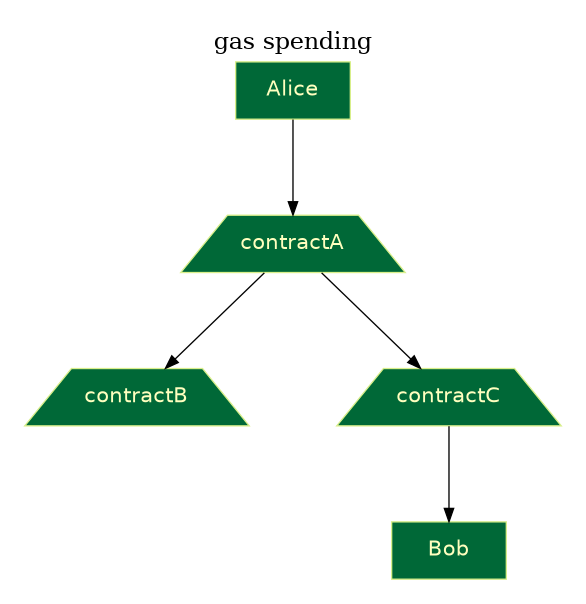
\includegraphics[scale=0.35]{gas}

\section{Solidity}

The Solidity language is a front-end to the EVM, offering a programming language
with java-like syntax that compiles to EVM bytecode.  Solidity enables
programming with two fundamental notions, accounts and transactions.  Accounts
cover human-owned wallets as well as generic smart contracts.  Transactions are
any communication between accounts.

\subsection{Memory}

There are two types of memory offered to the user, persistent and volatile.
Persistent memory keeps track of data across multiple contract invocations, and
is relatively expensive, partially because every miner on the blockchain must
keep track of it as well.  Volatile memory is a freshly cleared amount of memory
allotted to each contract at the beginning of each message call.

\subsection{Language Features}

The Solidity language offers a feature called ``require'' which acts like an
assert as in C/C++.  There is additionally a reserved function ``emit'' which
directly writes to the blockchain.  Moreover, there are several global variables
and functions that a contract might call out to, including ``gasLeft'',
``SHA256'' and ``keccak256''.

There are also several function visibilities.  These are keywords that constrain
who may invoke a given function.  

\begin{enumerate}
\item external: functions marked ``external'' may only be called from outside the contract
\item public: anyone may invoke these functions
\item private: such functions may only be used from within the defining contract
\item internal: may be used by the defining contract as well as derived contracts
\item view: these functions may only read storage
\item pure: these functions do not touch storage whatsoever
\end{enumerate}

\subsection{Code Reuse}

There are two unique ways in which contracts can be reused, revolving around an
import mechanism, similar in spirit to the import statement in Python or Haskell.
The first style is termed ``inheritance'', and involves using other contracts as
pre-compiled bytecode directly in a contract.  This is commonly done with the
SafeMath contract, which provides exception-free commonly used mathematical functions.
The second style uses other contracts as libraries, which are not pre-compiled.  

\subsection{Types}

Solidity contains several base types, including uint256, byte32, bool, and
address literals that are used to hold hashes but may not be used in arithmetic.

There are also reference types, including structs, arrays, strings, as well as
sort of constrained hash table called a ``mapping''.  

\section{ERC20 Tokens}

Solidity contracts have a strong tendency to describe financial instruments and
related constructions.  To this end, there was an Ethereum Improvement Proposal
that created a standard template for fungible tokens.  The template describes
ERC20 tokens and provides a standard API for transfering and spending such
tokens.  It is a very commonly reused contract in the Ethereum ecosystem.

\subsection{ABI}

Fundamentally, the fact that Solidity offers multiple programming features that
encourage writing safe, minimal code is irrelevant if the core bits that are
being exchanged in these complicated transactions cannot be agreed upon.  This
fact put the concept of ABI or Application Binary Interface at the forefront of
Solidity's design.  The ABI is a lower level description of functions (than say,
an API), which explains how functions will exactly behave at the byte level.  

\section*{References}
\beginrefs

\bibentry{Sol} ``Solidity, v0.7.4``. [Online]. Available: https://solidity.readthedocs.io/en/v0.7.4/index.html''.  Accessed on: Nov. 2, 2020.

\endrefs

% **** THIS ENDS THE EXAMPLES. DON'T DELETE THE FOLLOWING LINE:

\end{document}

